\section{Results}
\label{sec:results}


Figures~\ref{fig:plots:fashion-mnist-scaling}A, ~\ref{fig:plots:glove-25-scaling}B, and ~\ref{fig:plots:sift-scaling}C show the scaling behavior of CAKES on augmented versions of the following ann-benchmark datasets: fashion-mnist under Euclidean distance, glove-25 under cosine distance, and sift under Euclidean distance. 
Figure~\ref{fig:plots:random-scaling}D shows the scaling behavior of CAKES on a completely randomly generated dataset with same cardinality and dimensionality as sift (1 million points in 128 dimensions).
The horizontal axis in each figure denotes the multiplier by which we increased the cardinality of the original dataset with synthetic points (see Section \ref{subsec:methods:synthetic-data}). 
The vertical axis denotes throughput in queries per second. Both axes are on a logarithmic scale. In this section, we discuss results only for $k$-NN search with $k = 10$, but similar plots for $k=100$ can be found in our Supplement section. In these plots, we label the recall at each scale for algorithms which do not exhibit perfect recall; if no such labels are given for an algorithm, then that algorithm exhibits perfect recall at all scales.

Tables \ref{table:results:ann-fashion}, \ref{table:results:ann-glove-25}, \ref{table:results:ann-sift}, and \ref{table:results:ann-random} show the throughput and recall of CAKES's algorithms at each cardinality multiplier (i.e., scale) for the fashion-mnist, glove-25, sift, and random datasets respectively. When reporting recall, we use 1.000* to denote that the recall is imperfect, but rounds to 1.000 when we consider
only three decimal places.

In Figure~\ref{fig:results:fashion-mnist-scaling}, which shows results for fashion-mnist, we observe that as the augmentation multiplier increases, the CAKES algorithms (GreedySieve in blue, RepeatedRnn in green, and Sieve in red) exhibit higher throughput than na\"{i}ve linear search, plotted in orange. We also observe that CAKES outperforms state-of-the-art similarity search algorithm FAISS-Flat (plotted in brown) for all cardinality multipliers and outperforms FAISS-IVF (plotted in pink) for all multipliers greater than $10^{5.5}$. Though state-of-the-art algorithms HNSW (plotted in gray), and Annoy (plotted in purple) have higher throughput than CAKES for all multipliers, we note that CAKES exhibits perfect recall for all multipliers, while hnsw and annoy exhibit much lower recall, as shown in Table~\ref{table:results:ann-fashion}. For example, at a cardinality multiplier as low as eight, hnsw and annoy have recall of 0.525 and 0.857 respectively, while CAKES exhibits perfect recall.
Amongst the CAKES algorithms, GreedySieve consistently performs best on this dataset, exhibiting sublinear time performance for nearly all cardinality multipliers. 


With glove-25 (Figure~\ref{fig:results:glove-25-scaling}), we observe that each of CAKES' algorithms outperforms linear search at high cardinality multipliers. Similar to the results for fashion-mnist, we observe that CAKES outperforms FAISS-Flat for all cardinality multipliers and outperforms FAISS-IVF for all multipliers greater than $10^{7}$. We also see that while hnsw and annoy have higher throughput than CAKES for all multipliers, CAKES exhibits perfect recall for all multipliers, while hnsw and annoy exhibit much lower recall, as shown in Table~\ref{table:results:ann-glove-25}. For example, at a cardinality multiplier as low as eight, hnsw and annoy have recall of 0.294 and 0.857 respectively, while CAKES exhibits perfect recall.
On this dataset, Repeated $\rho$-NN, plotted in green, is consistently the best-performing algorithm. {\color{red} Revive lfd violin plots to add explanation for this.}


In Figure~\ref{fig:results:sift-scaling}, we observe that while linear search performs best for low cardinality multipliers, our algorithms begin outperforming linear search beginning at a multiplier of approximately 7. 
For this dataset, Sieve, plotted in red, is the highest throughput algorithm for all multipliers greater than 7. 

Figure \ref{fig:results:random-scaling} displays results for a random datset with the same dimensionality and cardinality as Sift (i.e., 128 and 1,000,000 respectively). 
These results illustrate the fact that \emph{ceteris paribus}, absent a manifold structure in the dataset, CAKES's algorithms do not begin to outperform linear search until the cardinality multiplier is around 10. 
Repeated $\rho$-NN shows significantly worse performance on this dataset relative to both the other algorithms and to its own performance on real datasets. 
This is unsurprising, given that Repeated $\rho$-NN relies on a low local fractal dimension around the query in order to quickly home in on the correct radius for $k$ hits. 
With a completely random dataset, whose average local fractal dimension will be near its embedding dimension, Repeated $\rho$-NN will iterate for longer before finding this correct radius. 

Notably, we observe that on all datasets, GreedySieve's throughput stays nearly constant as cardinality increases. This observation warrants further investigation, but it is especially promising given that GreedySieve consistently outperforms linear search for high cardinalities. 
% We also notice an interesting trend with Sieve and Sieve with Separate centers: for all datasets, at both values of $k$, both algorithms exhibit a sharp ``pivot point'' after which throughput starts to increase. 
% While we observe that this pivot point seems to be proportional to the value of $k$, as it often occurs at about a multiplier of 4 when $k=10$ and a mulitplier of 32 when $k=100$, the reason for this behavior requires further investigation.  
Finally, we reiterate that the variation in performance of our algorithms across different datasets and cardinalities support our use of an autotuning function to select the best choice of algorithm. 
% Currently, our autotuning function always uses $k=10$ for its determination, but our observation that the best algorithm often differs between small and large values of $k$ suggests that more sophisticated autotuning is necessary.


\begin{figure}
\begin{subfigure}[b]{0.4\textwidth}
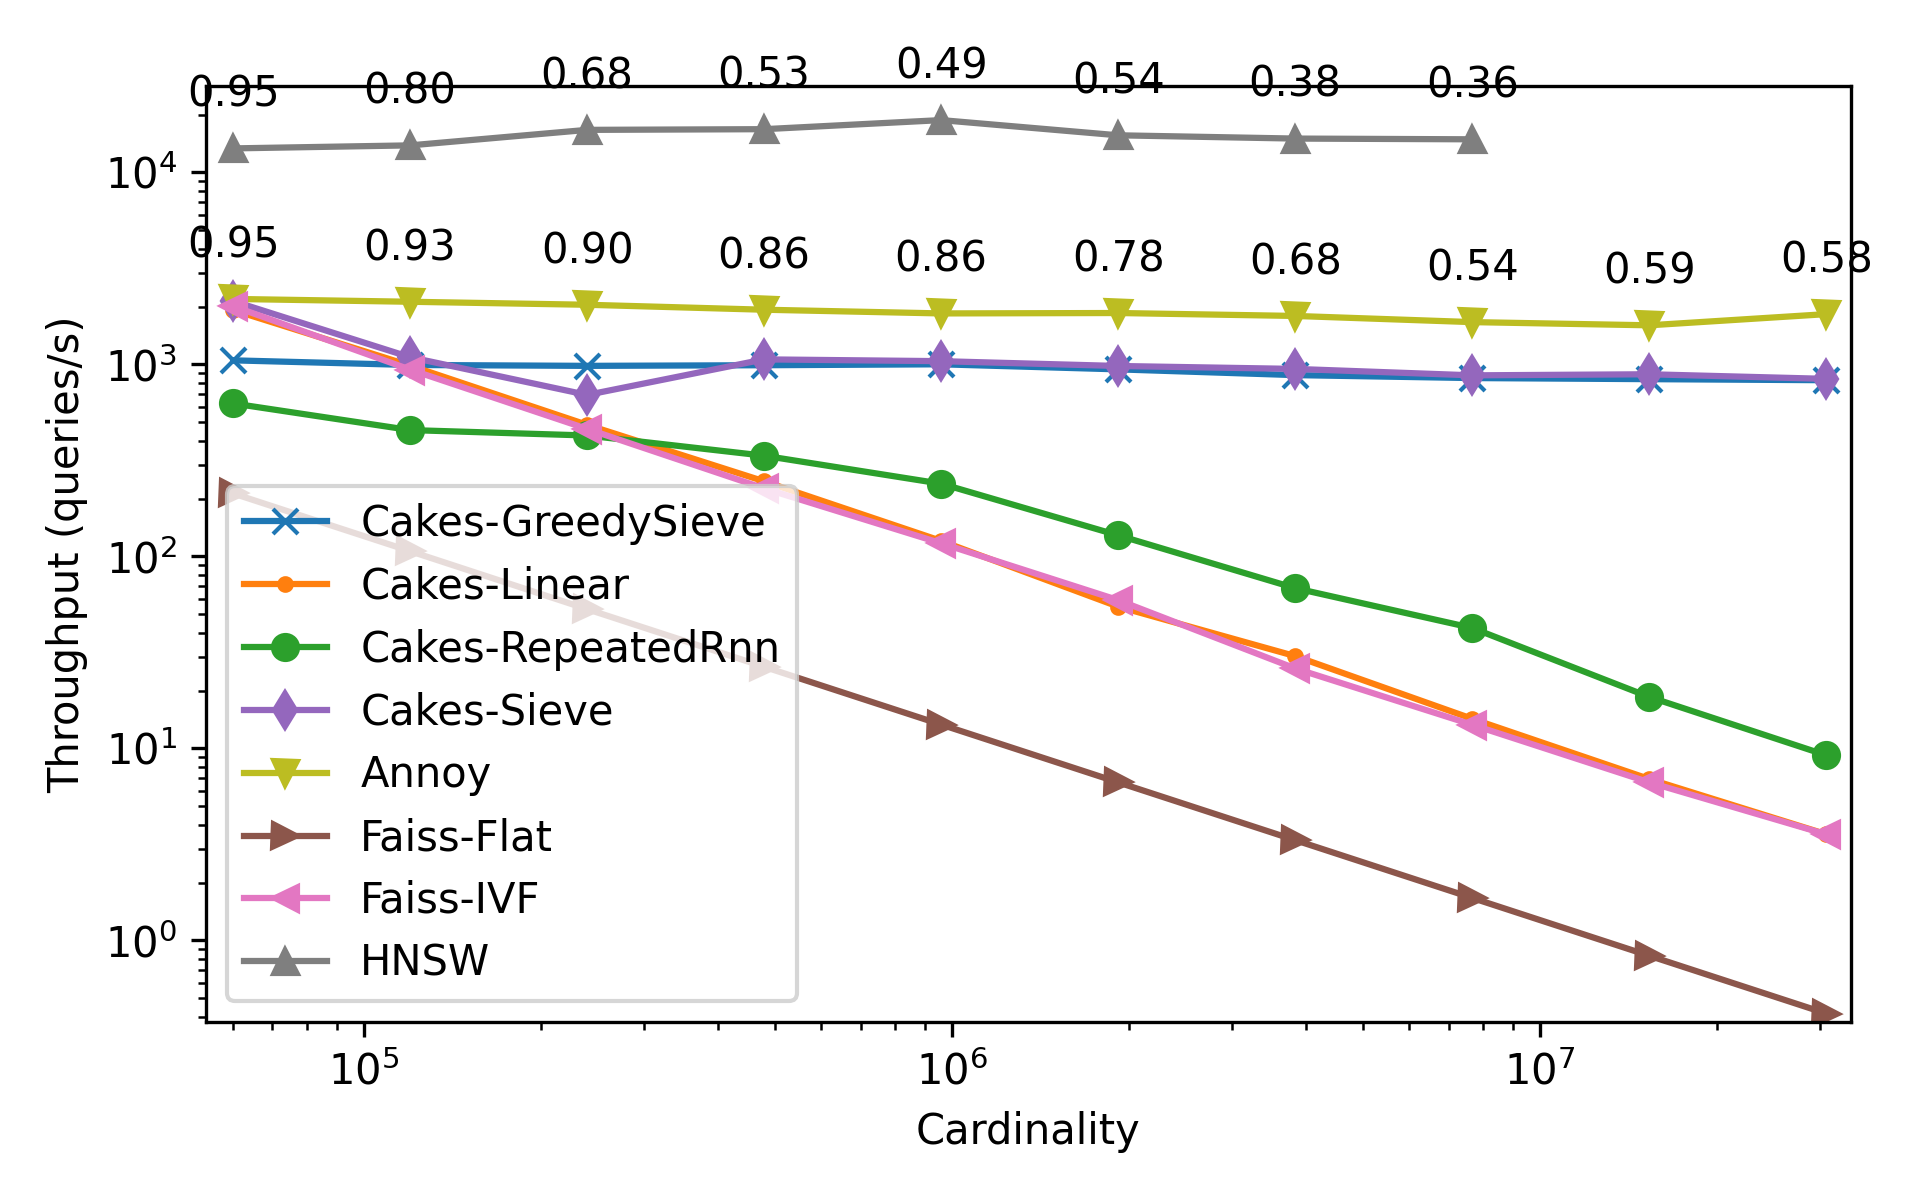
\includegraphics[width=0.95\textwidth]{plots/fashion-mnist-knn-10.png}\\
\subcaption{Fashion-mnist for $k=10$.}
\label{fig:results:fashion-mnist-scaling}
\end{subfigure}%
\begin{subfigure}[b]{0.4\textwidth}
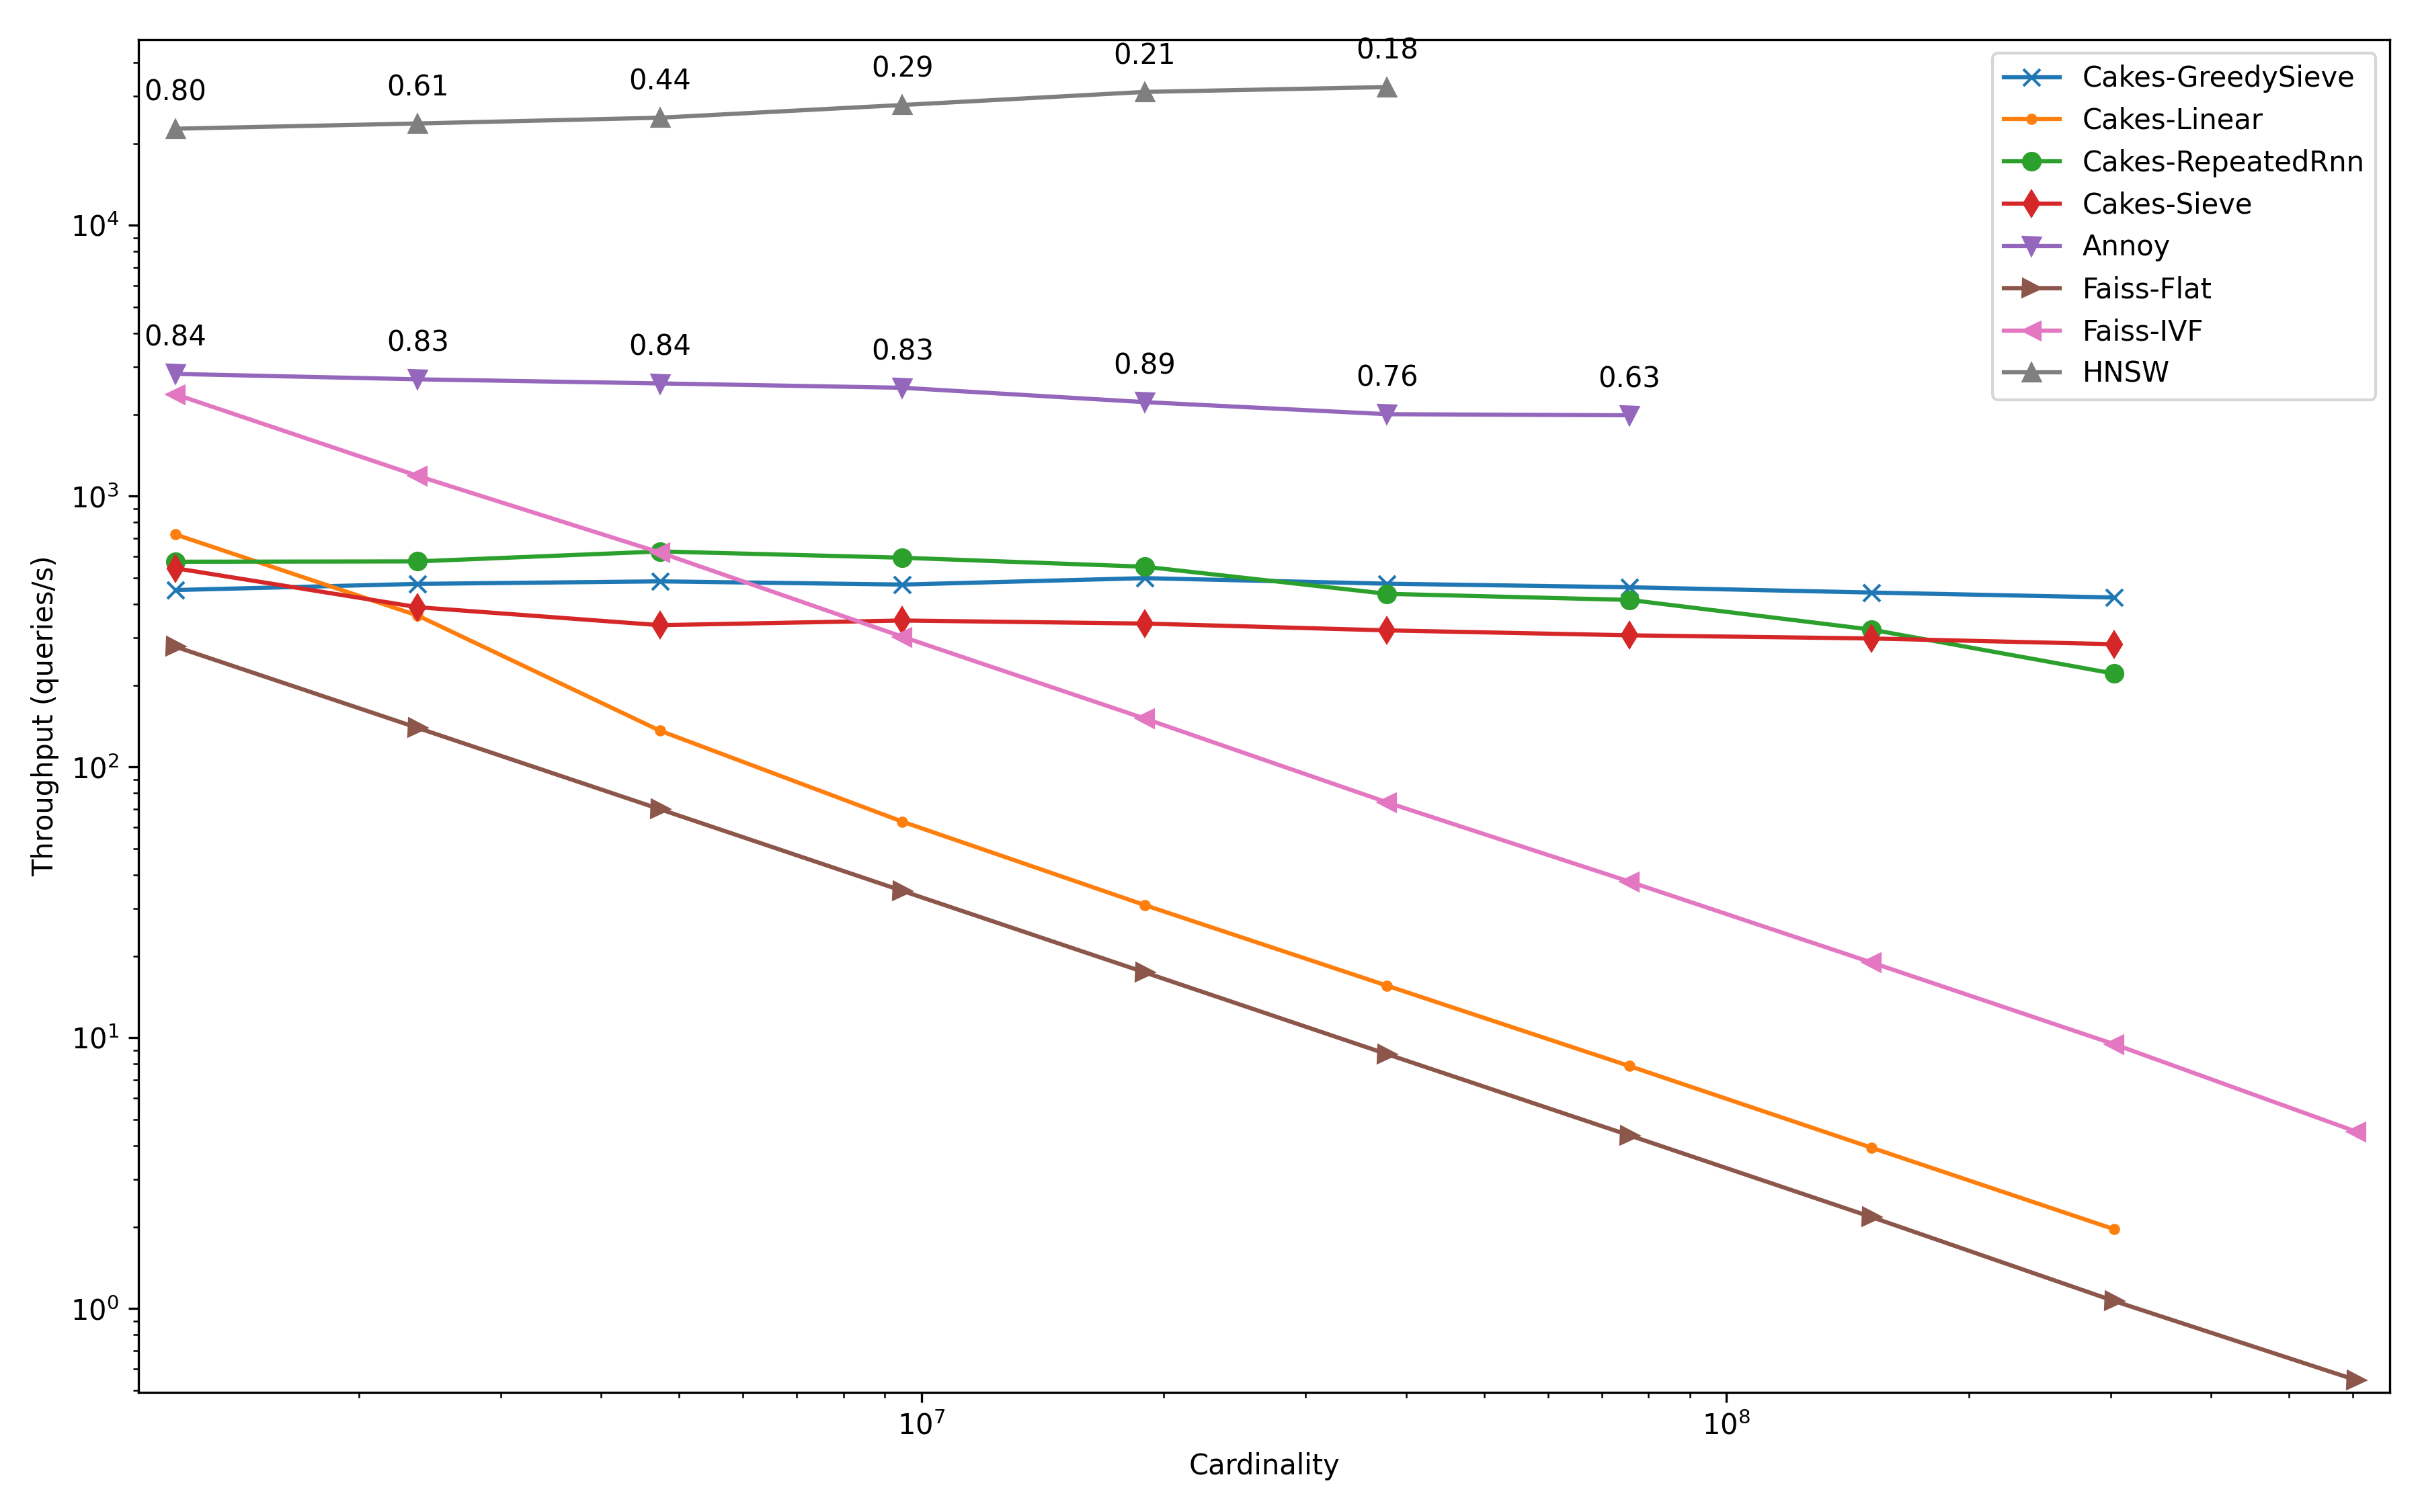
\includegraphics[width=0.95\textwidth]{plots/glove-25-knn-10.png}\\
\subcaption{Glove-25 for $k=10$.  }
\label{fig:results:glove-25-scaling}
\end{subfigure}%
\\
\begin{subfigure}[b]{0.4\textwidth}
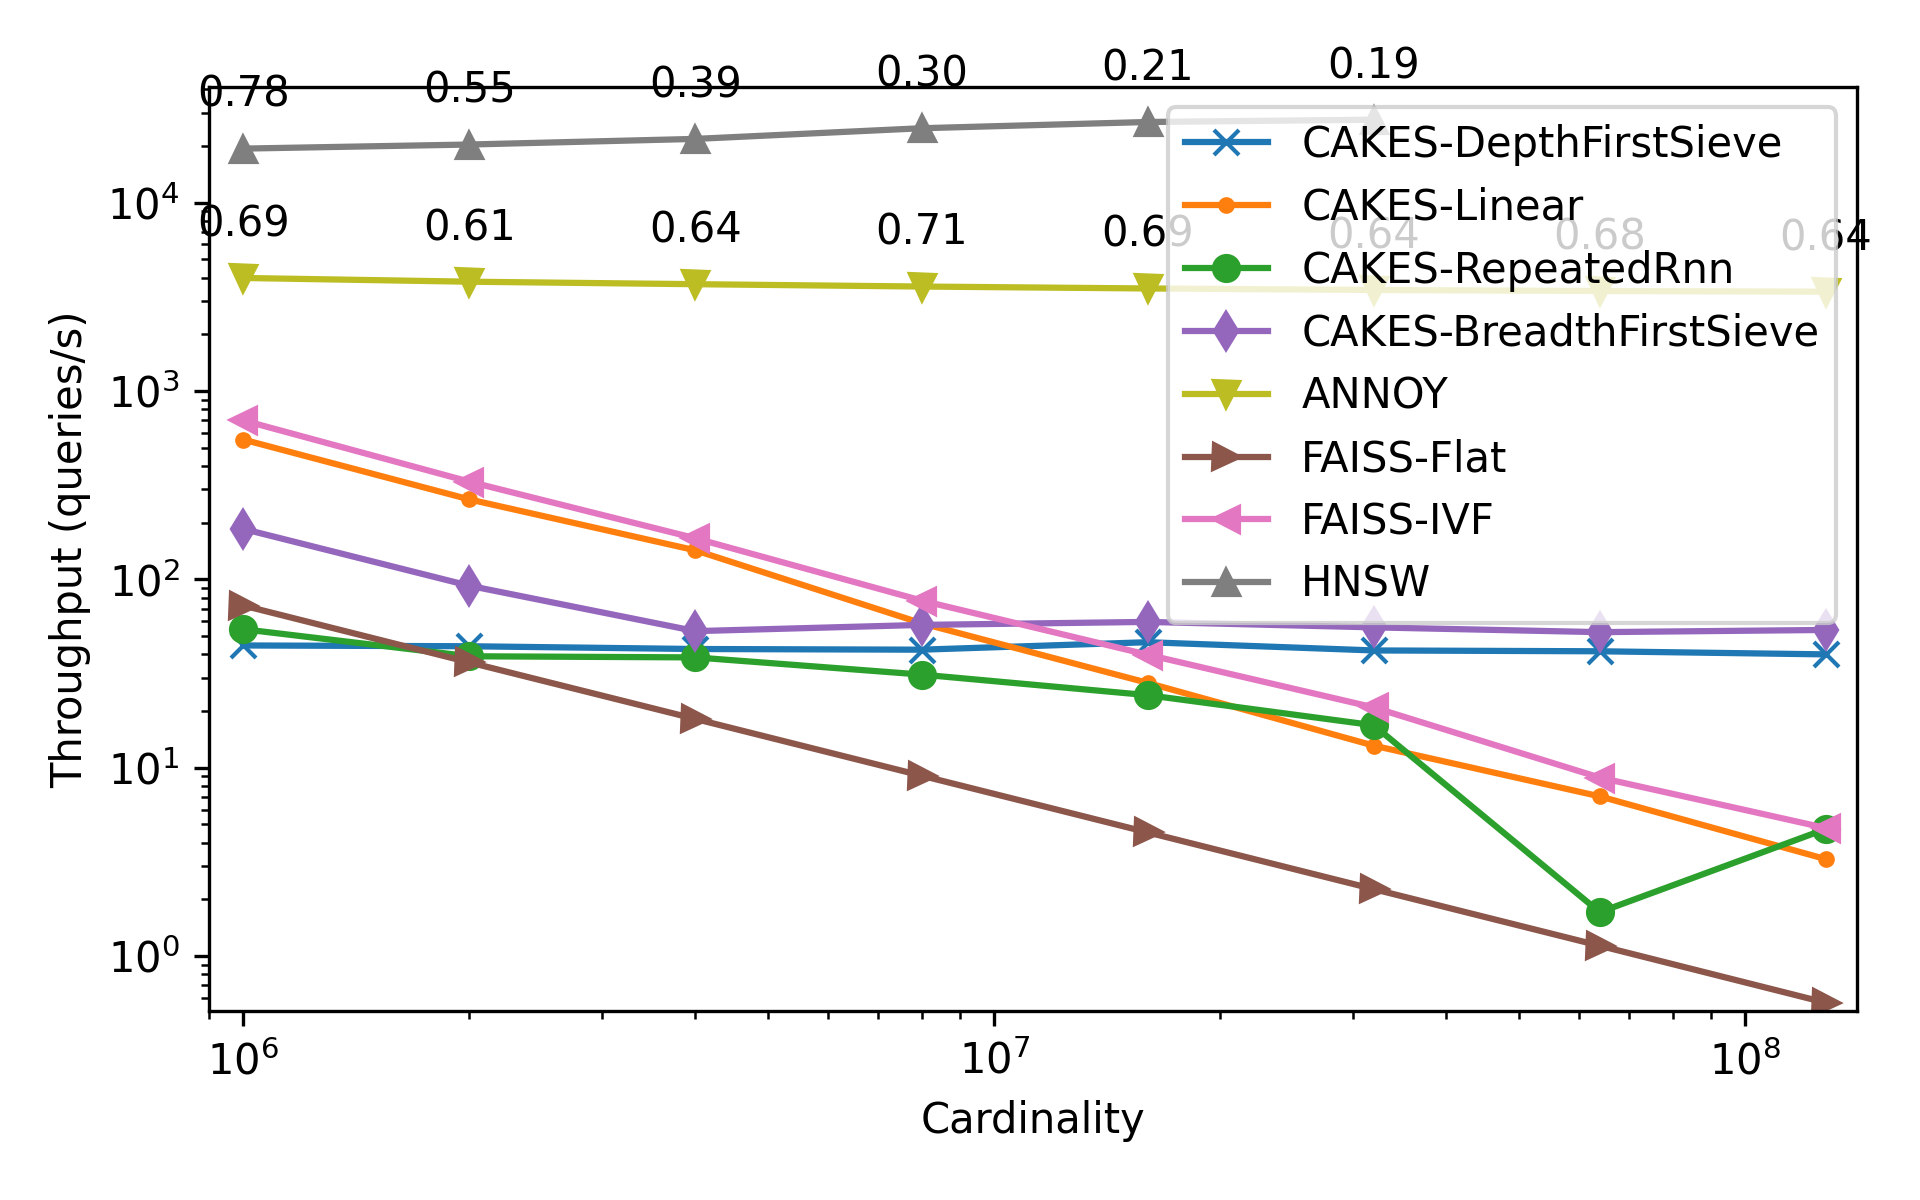
\includegraphics[width=0.95\textwidth]{plots/sift-knn-10.png}\\
\subcaption{Sift for $k=10$.    }
\label{fig:results:sift-scaling}
\end{subfigure}%
\begin{subfigure}[b]{0.4\textwidth}
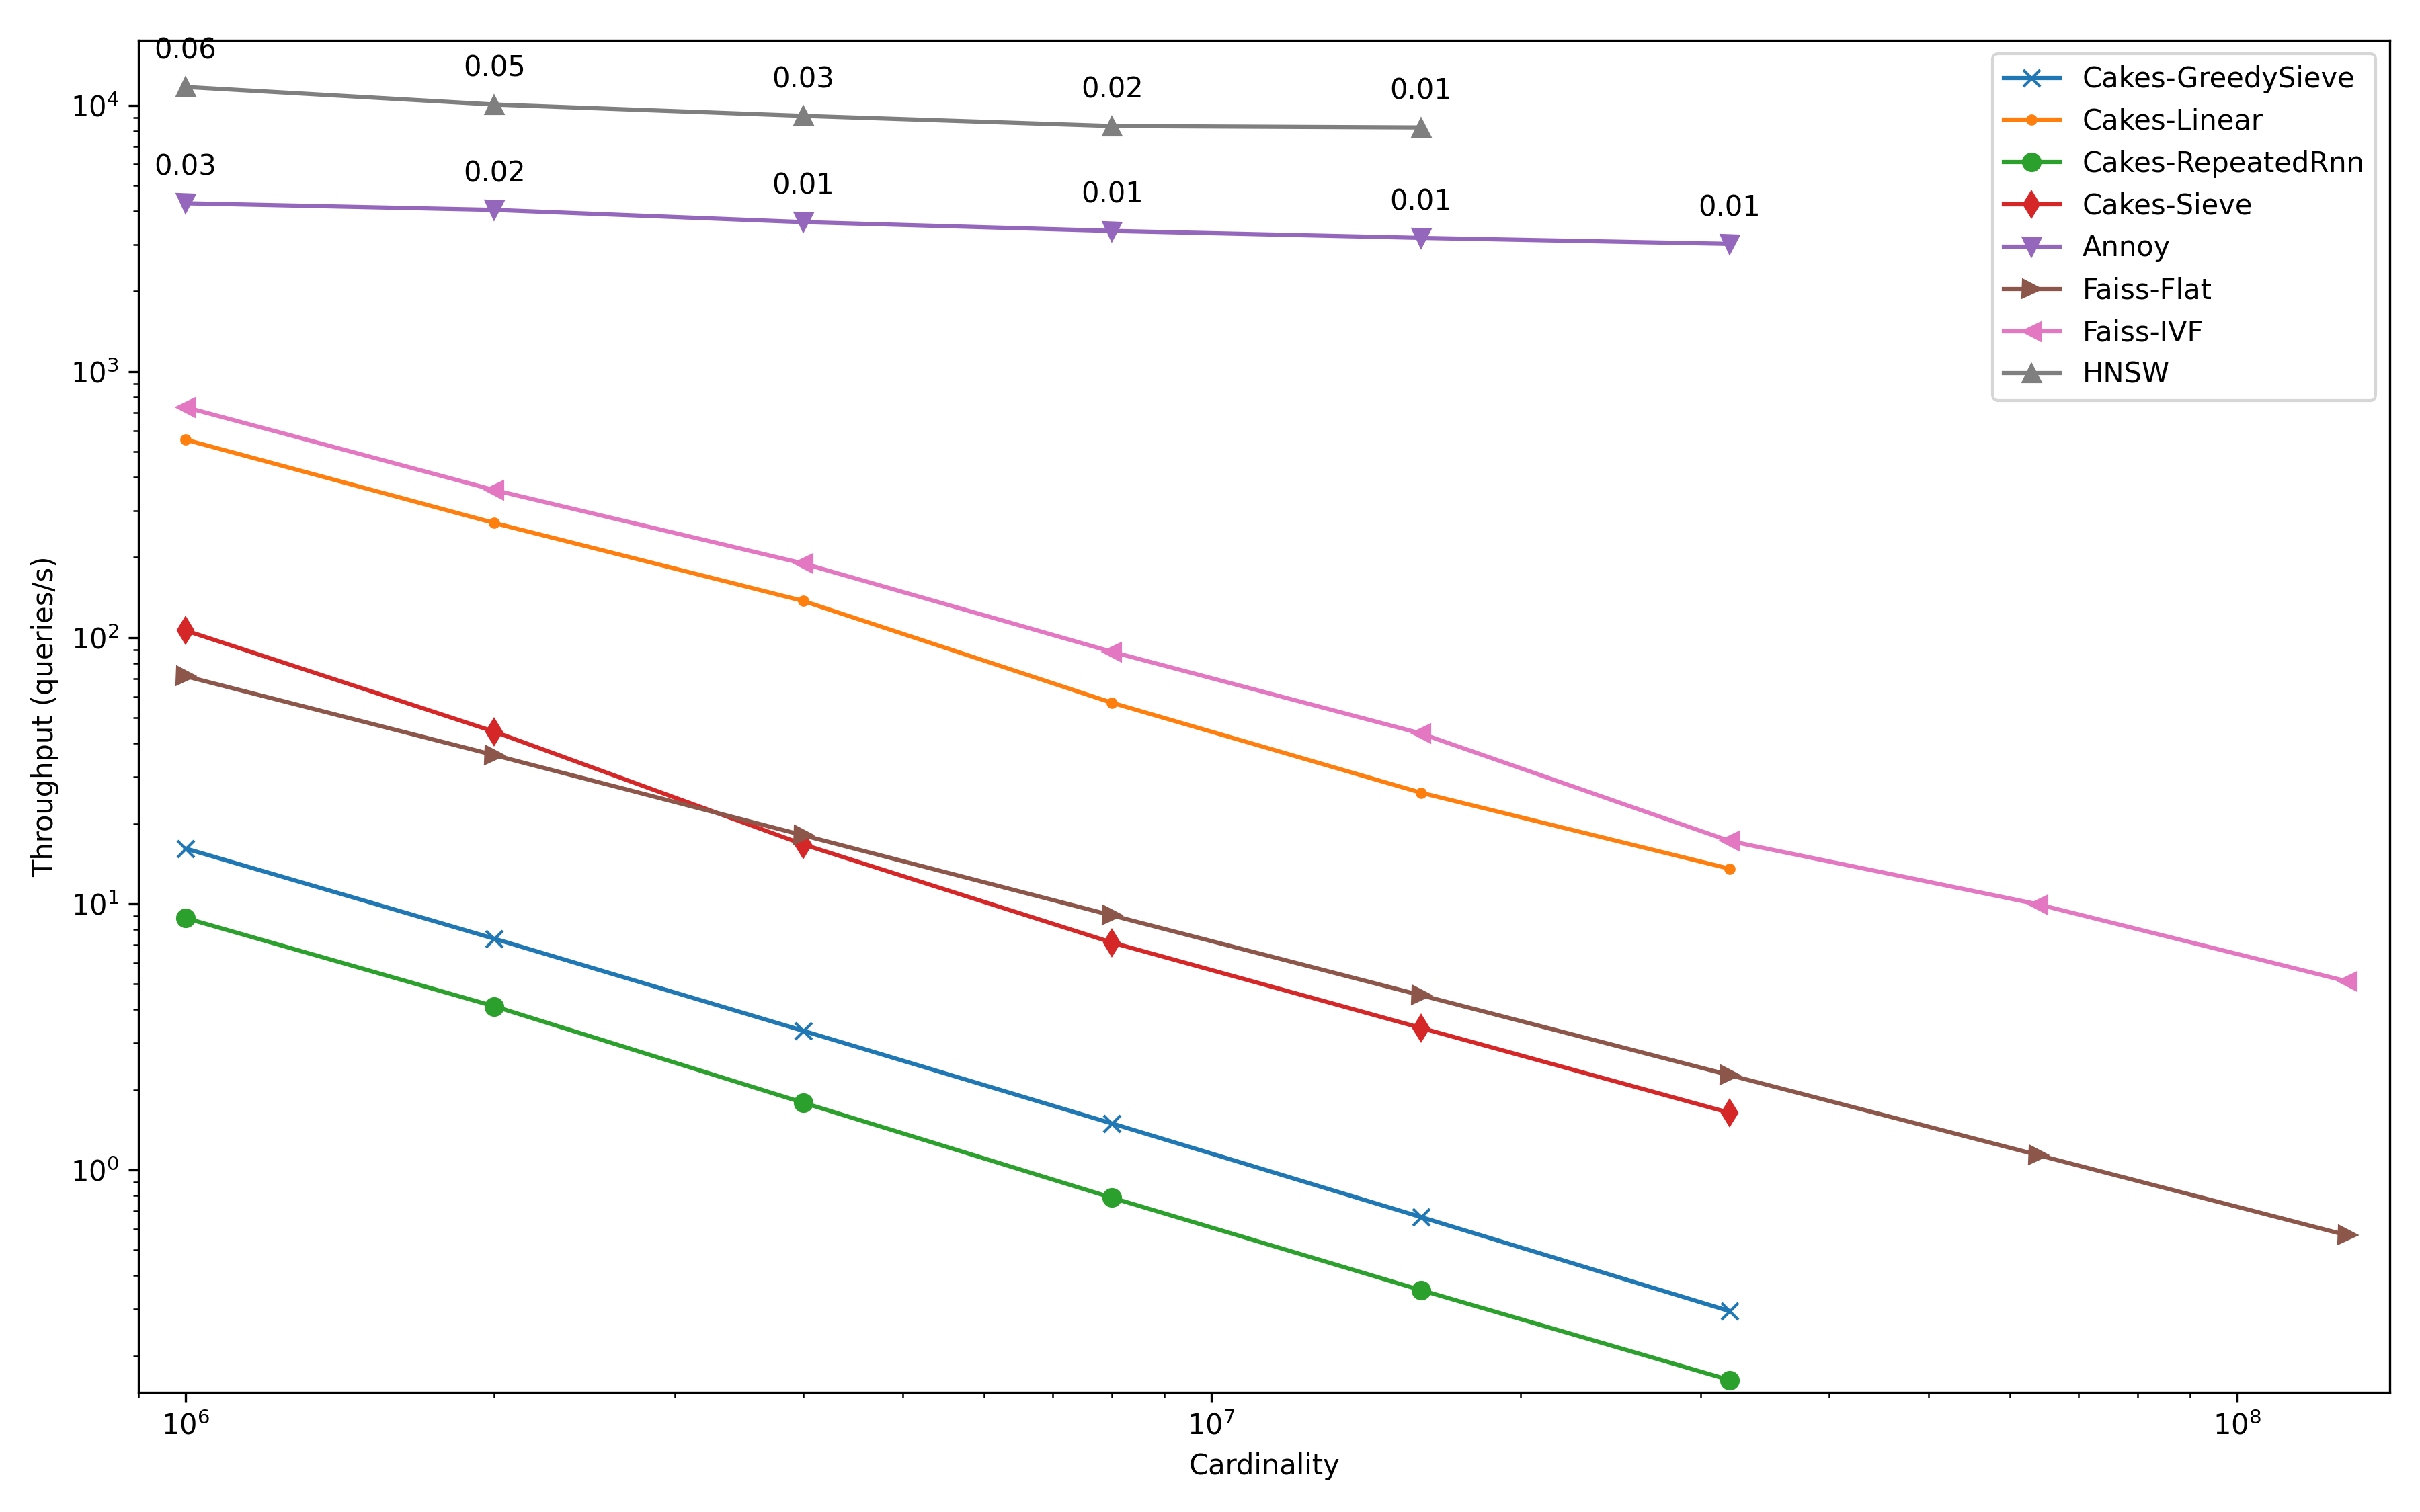
\includegraphics[width=0.95\textwidth]{plots/random-1000000-128-knn-10.png}\\
\subcaption{A random dataset for $k=10$.
}
\label{fig:results:random-scaling}
\end{subfigure}%

\caption{Algorithm performance across four datasets. In each plot, the horizontal axis represents increasing cardinality (size) of the dataset, while the vertical axis represents the throughput in queries per second (higher is better). TODO say something about plots that didn't finish.}
\end{figure}

% 
% \begin{figure}[ht!]
%     \centering
%     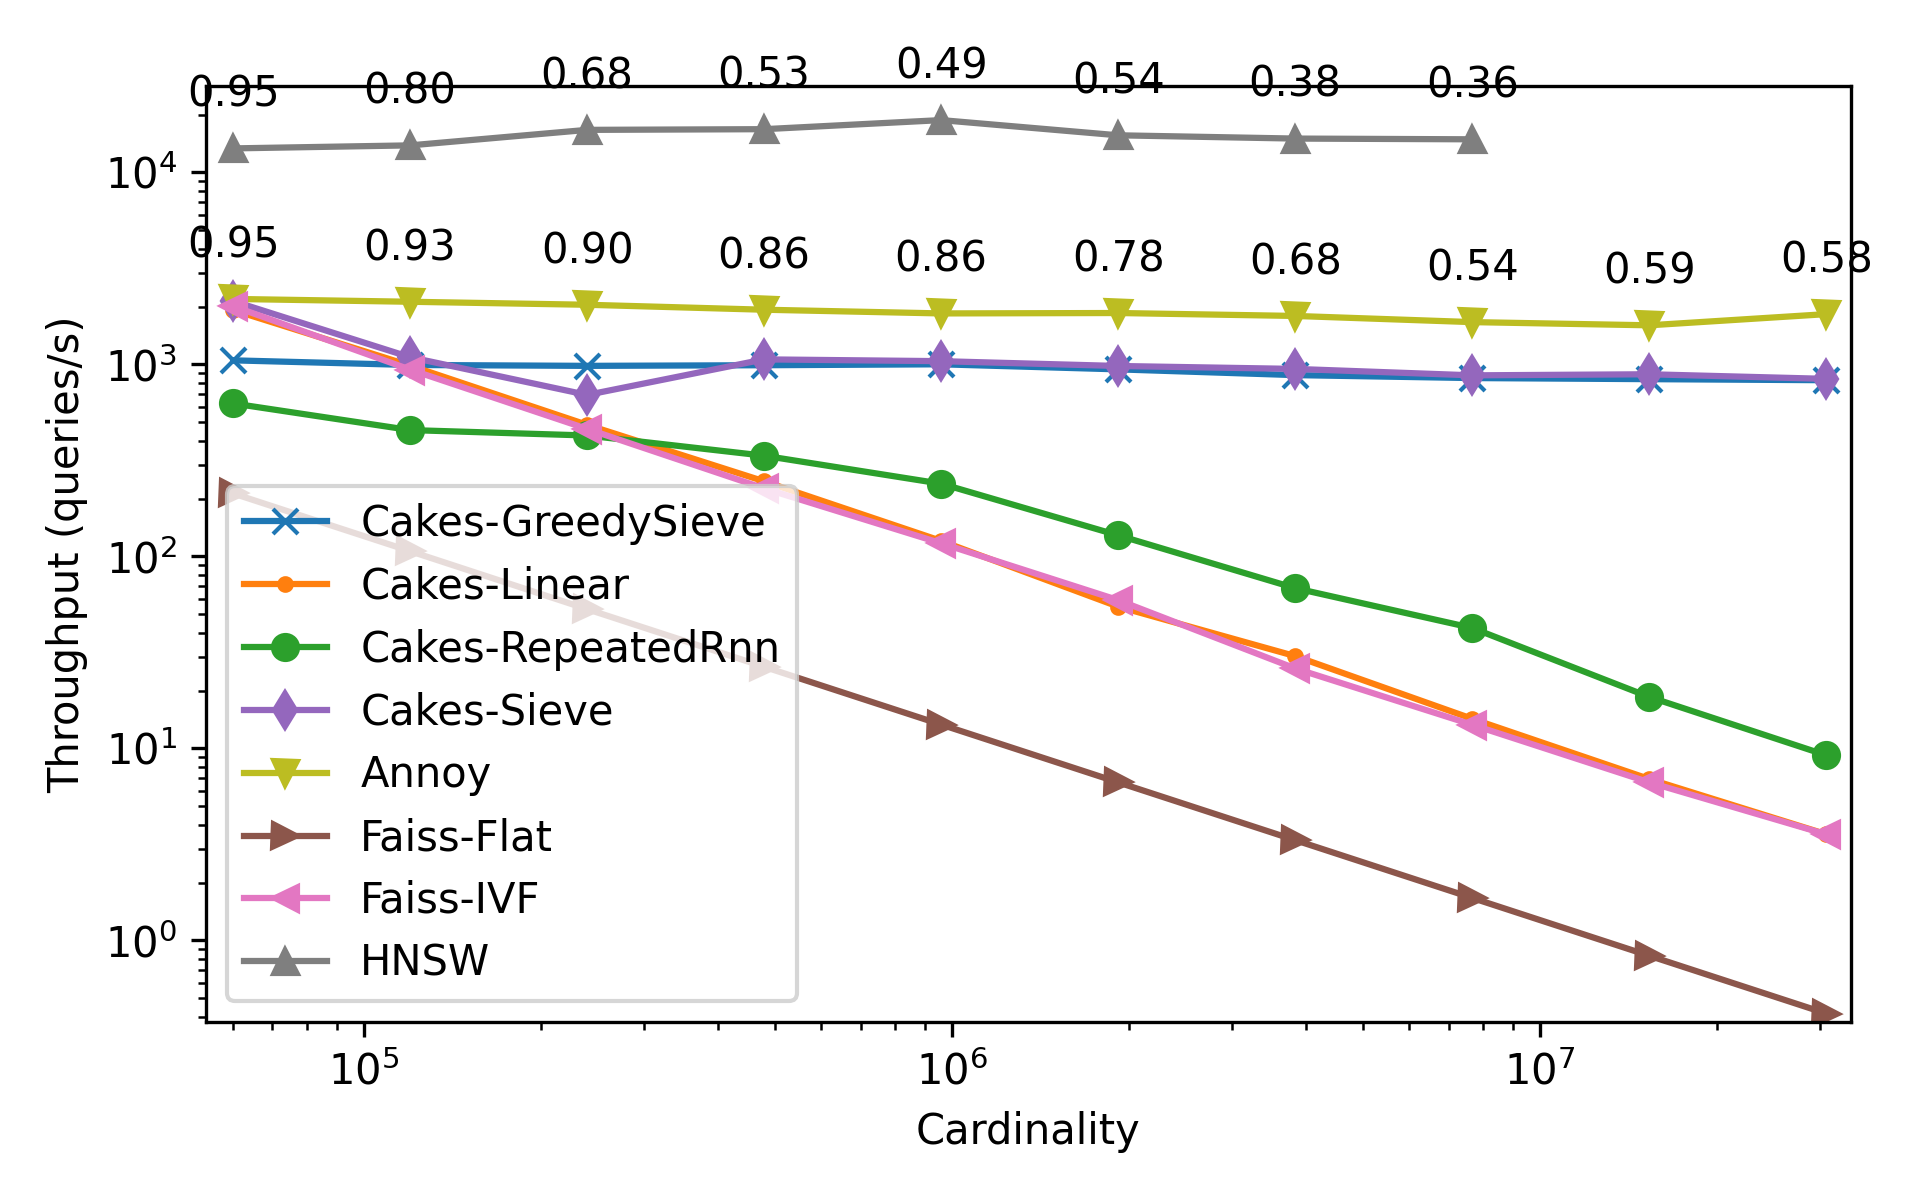
\includegraphics[width=3.4in]{plots/fashion-mnist-knn-10.png}
%     \caption{
%         Algorithm performance by cardinality multiplier on fashion-mnist for $k=10$.
%     }
%     \label{fig:results:fashion-mnist-scaling}
% \end{figure}

% \begin{figure}[ht!]
%     \centering
%     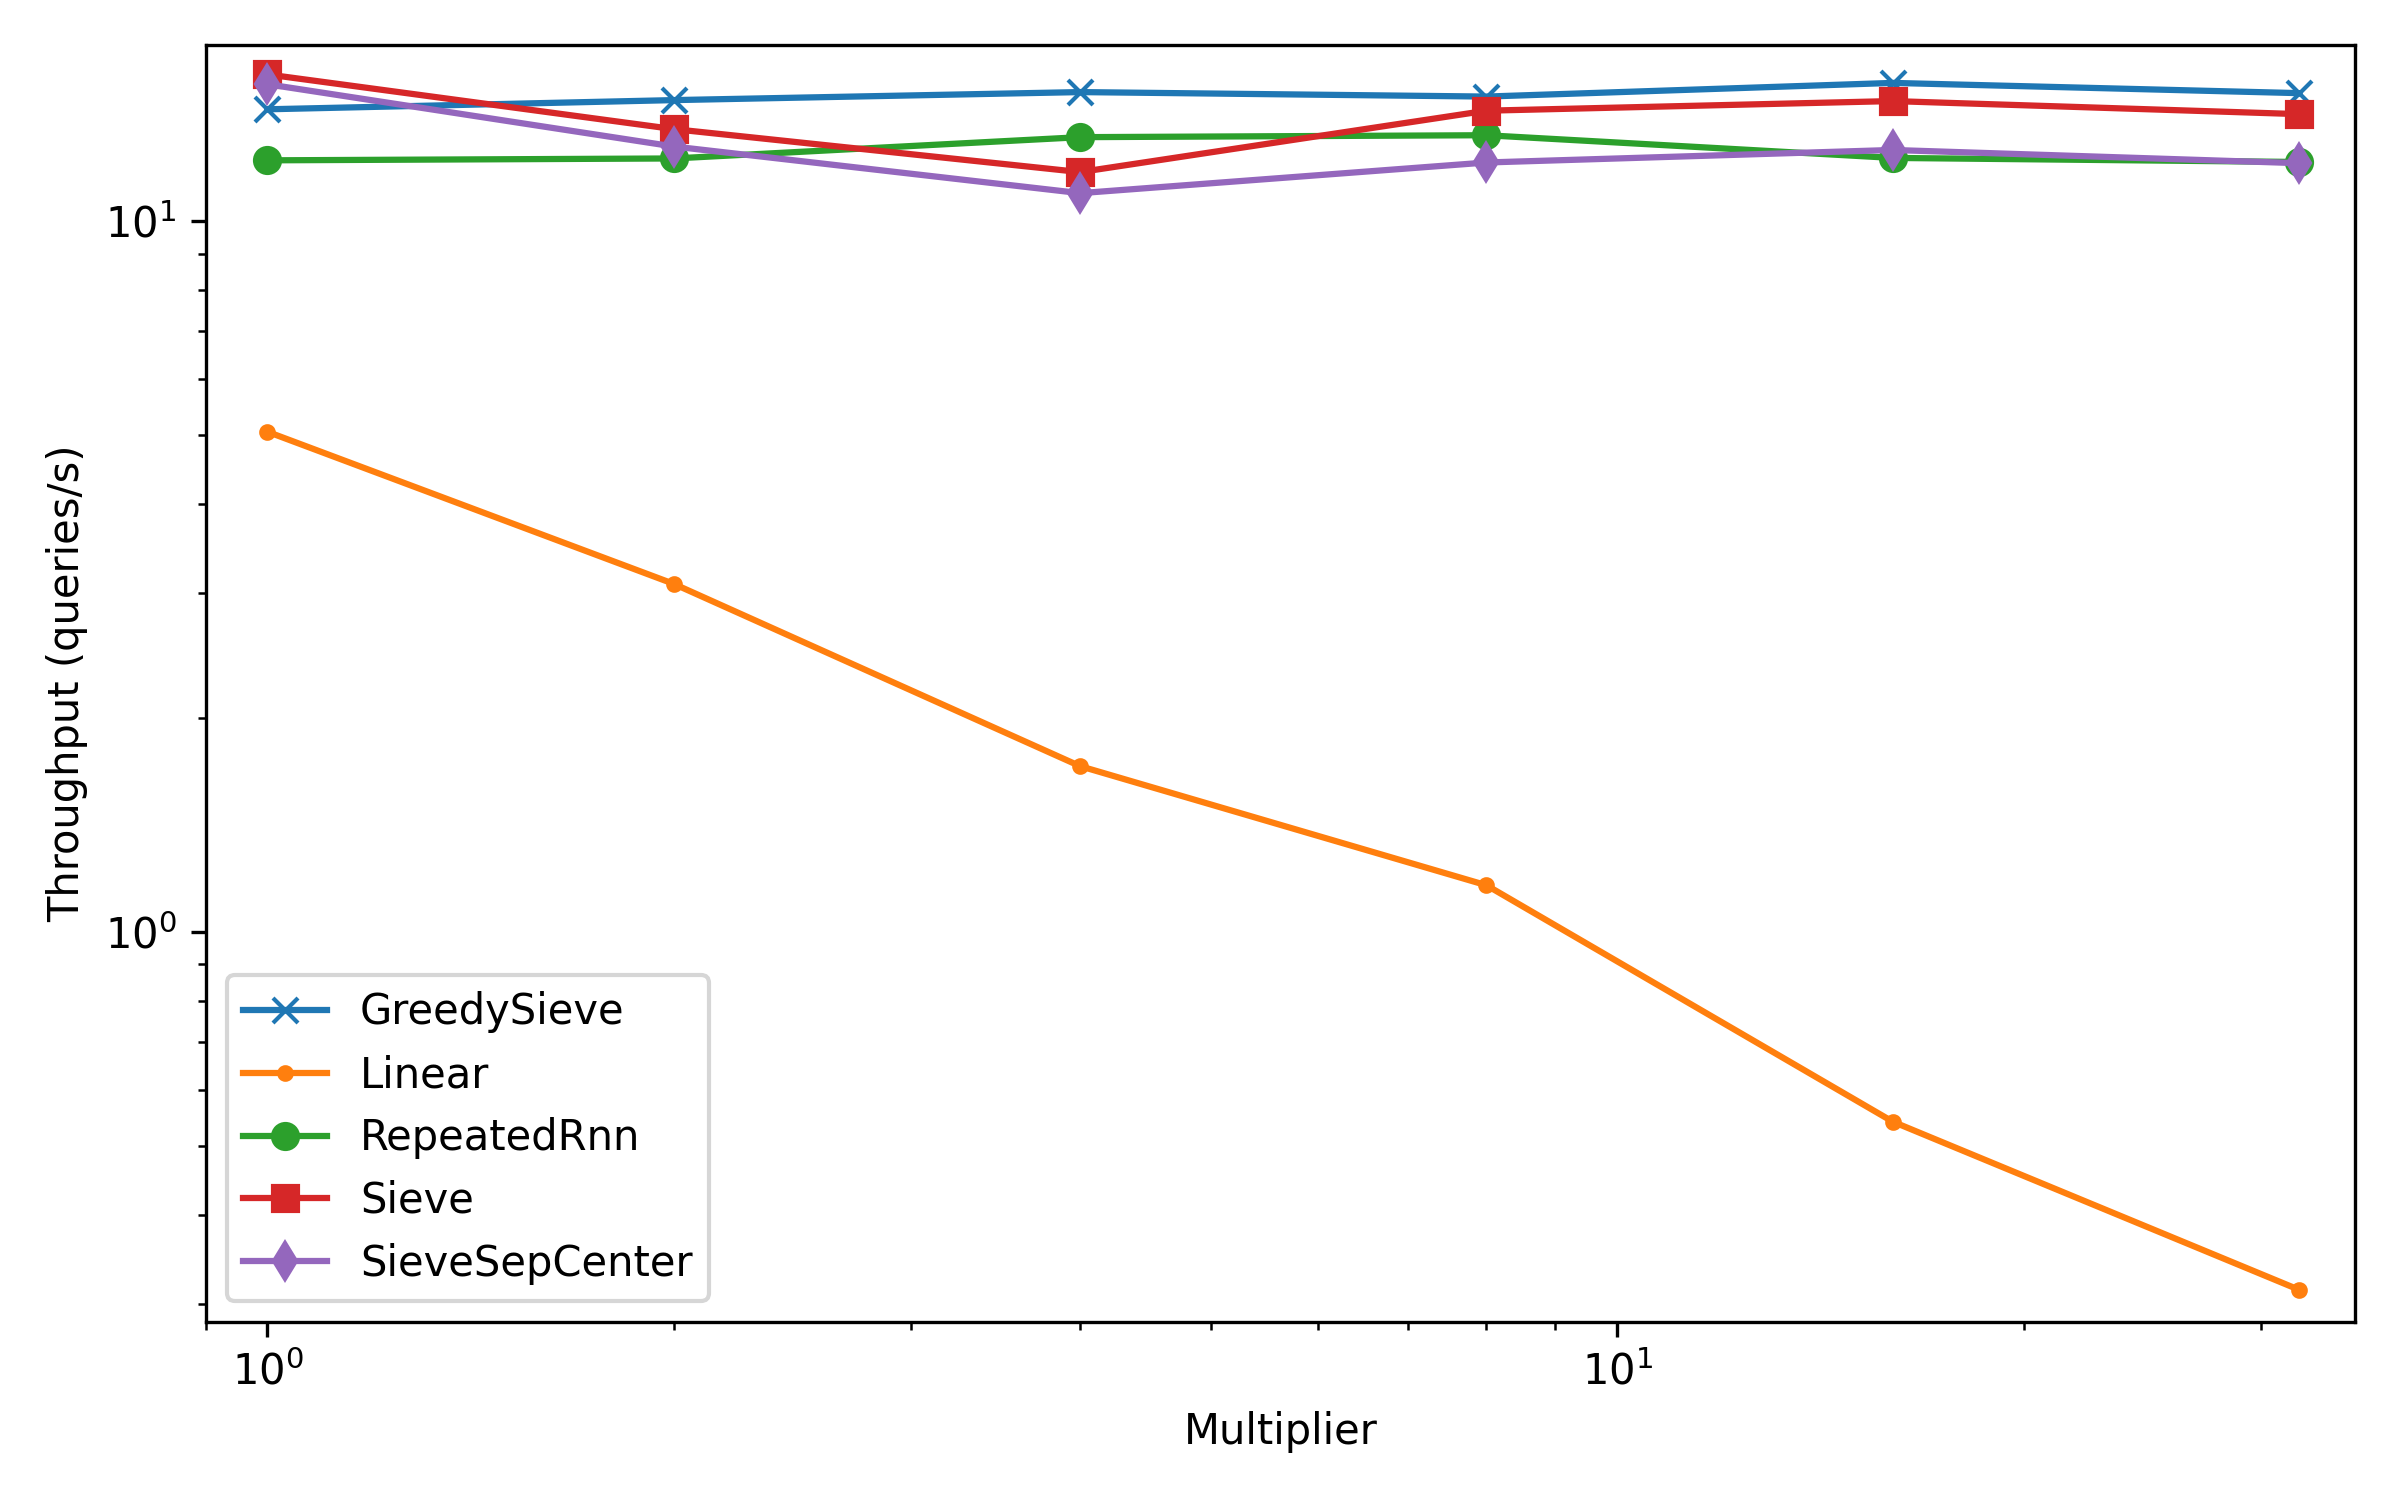
\includegraphics[width=3.4in]{images/result_plots/deep-image_10_scaling.png}
%     \caption{
%         Deep-image Scaling
%     }
%     \label{fig:results:deep-image-scaling}
% \end{figure}


% \begin{figure}[ht!]
%     \centering
%     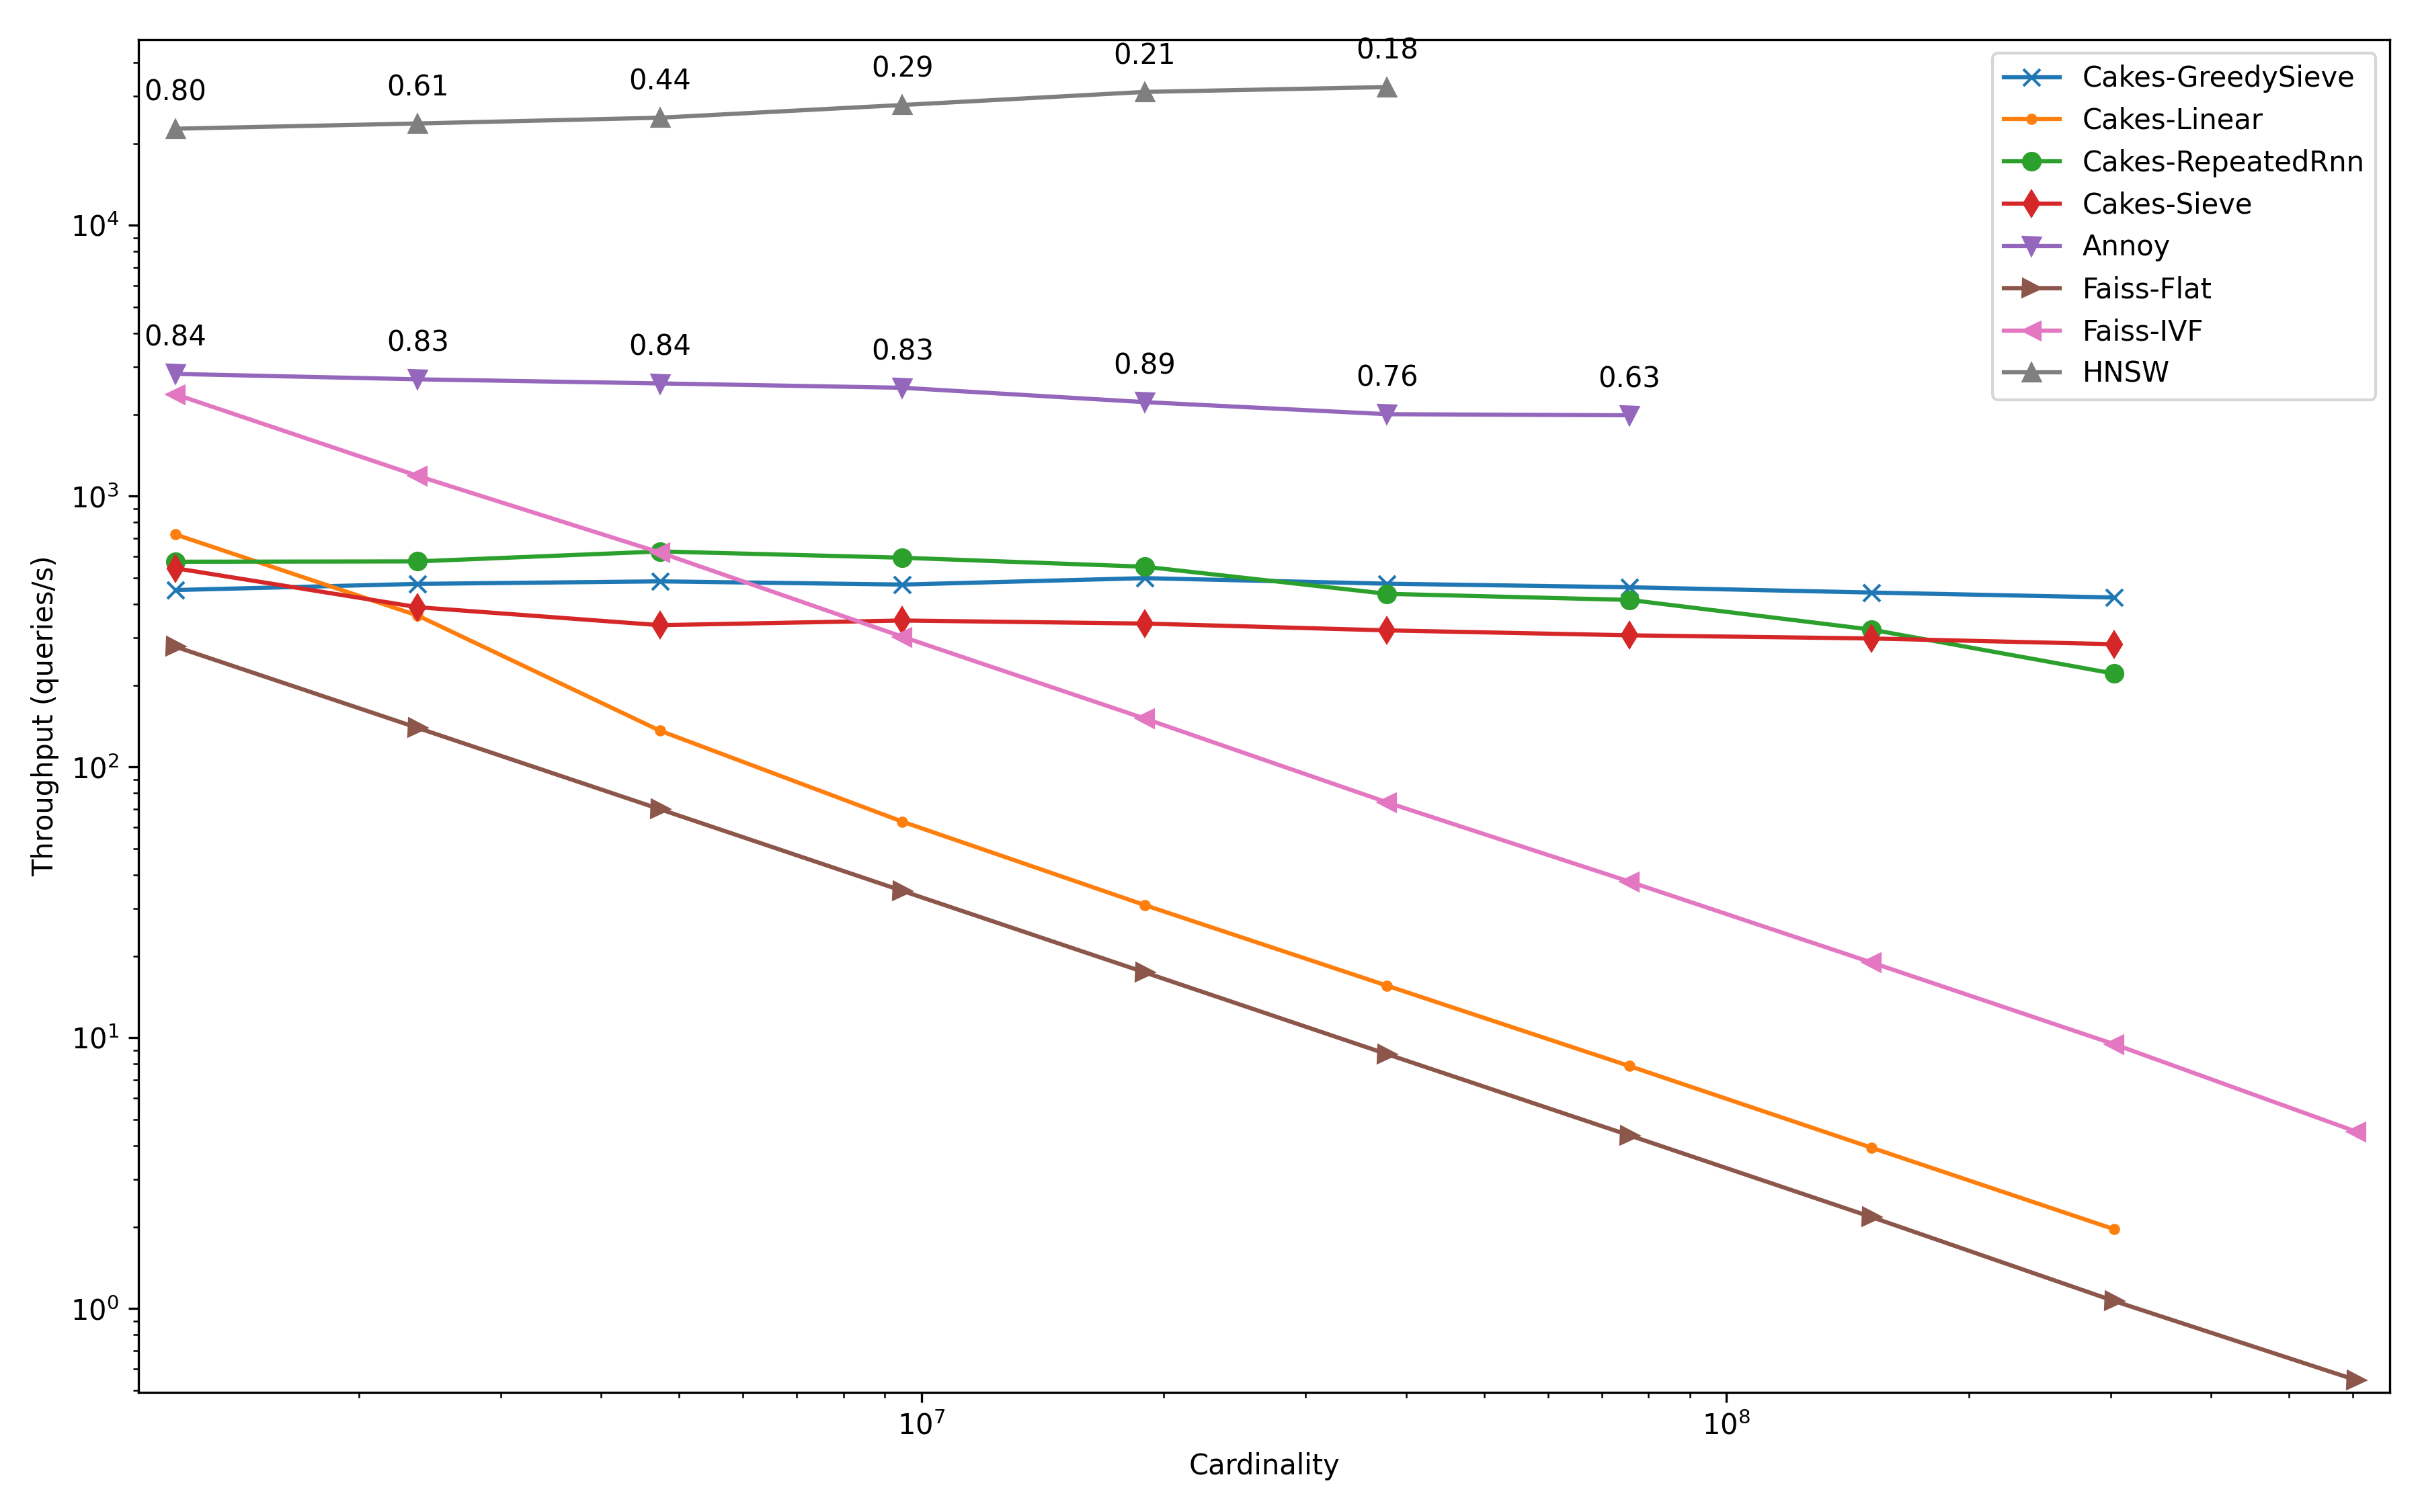
\includegraphics[width=3.4in]{plots/glove-25-knn-10.png}
%     \caption{
%         Algorithm performance by cardinality multiplier on glove-25 for $k=10$.  }
%     \label{fig:results:glove-25-scaling}
% \end{figure}

% 
% \begin{figure}[ht!]
%     \centering
%     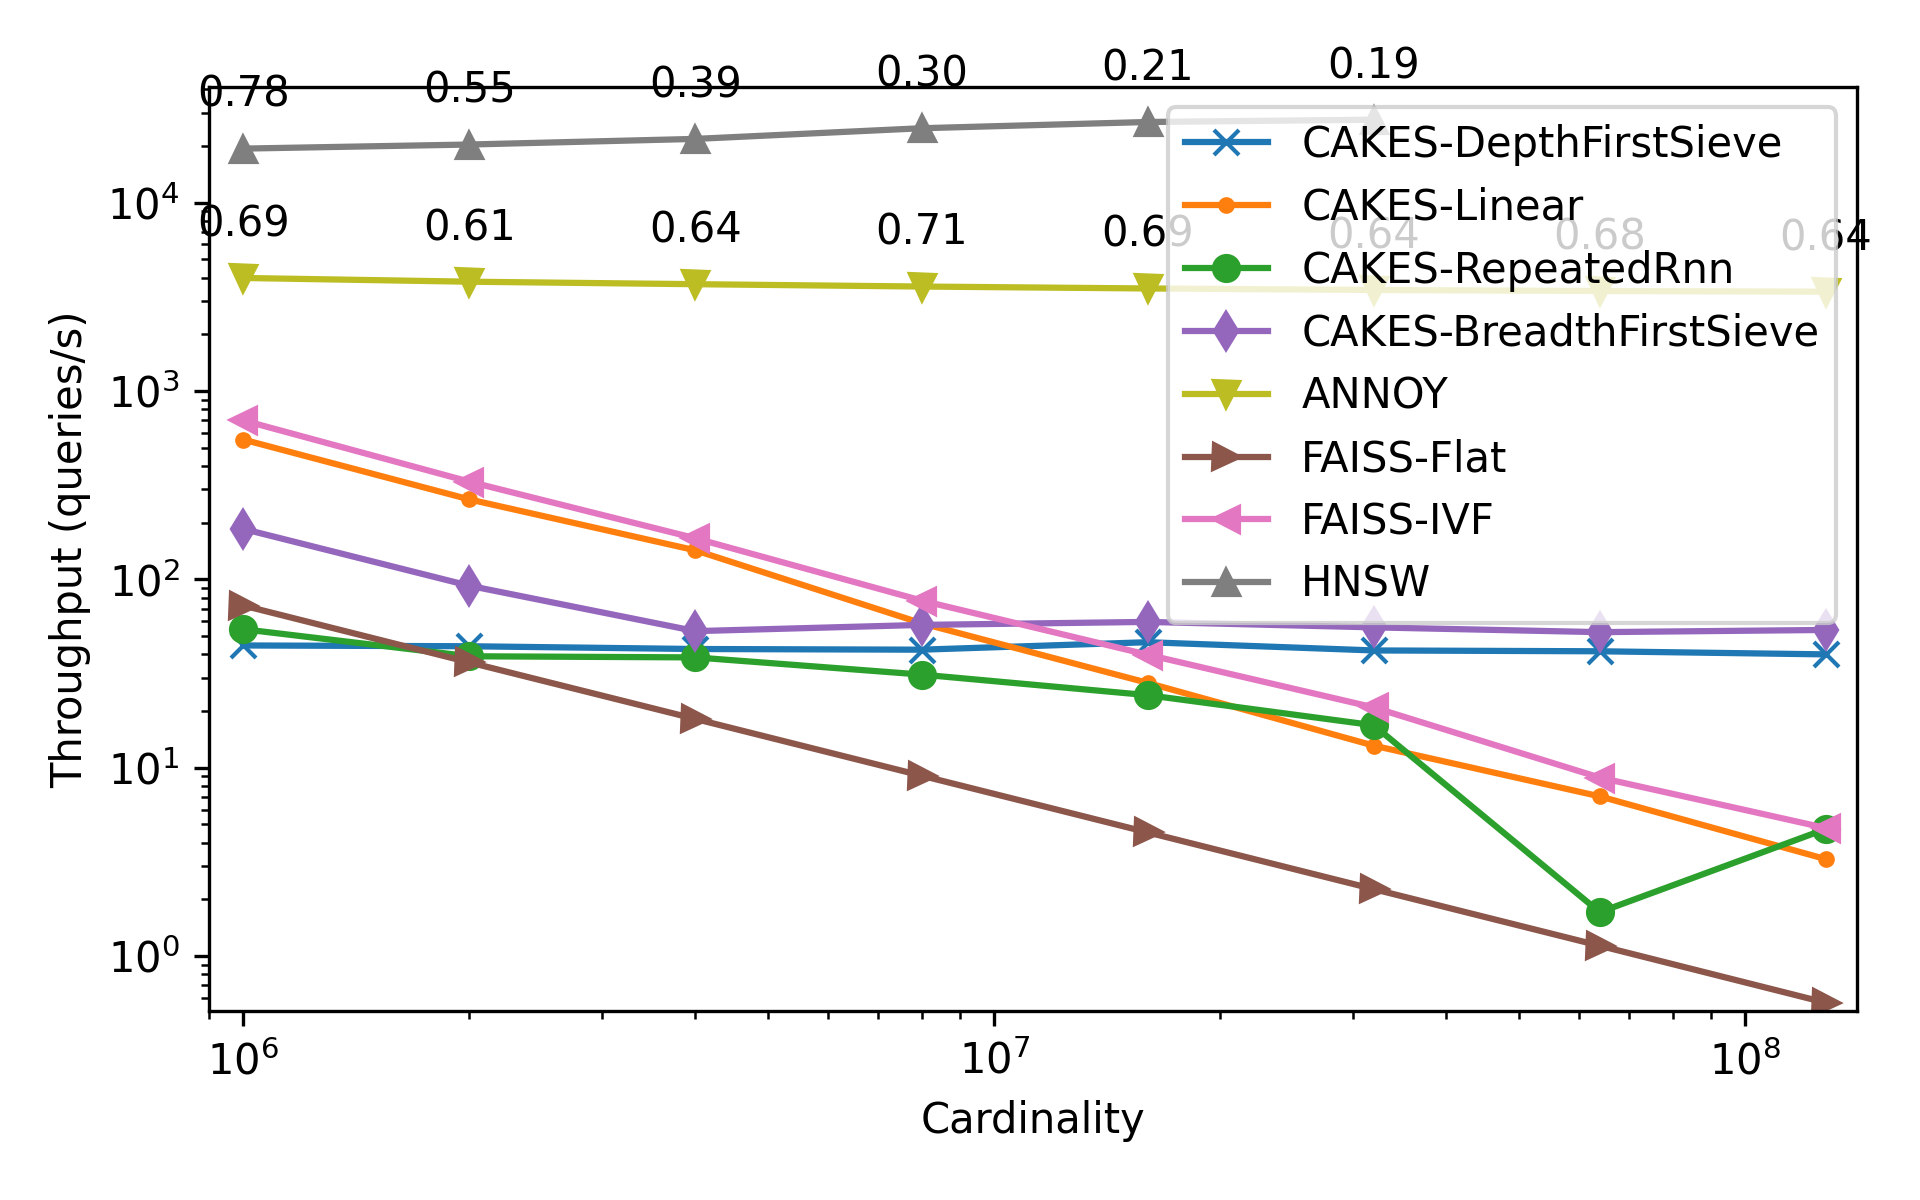
\includegraphics[width=3.4in]{plots/sift-knn-10.png}
%     \caption{
%         Algorithm performance by cardinality multiplier on sift for $k=10$.    }
%     \label{fig:results:sift-scaling}
% \end{figure}

% We need to redo this plot so that we do not actually augment random datasets but instead take larger and larger 
% random datasets
% 
% \begin{figure}[ht!]
%     \centering
%     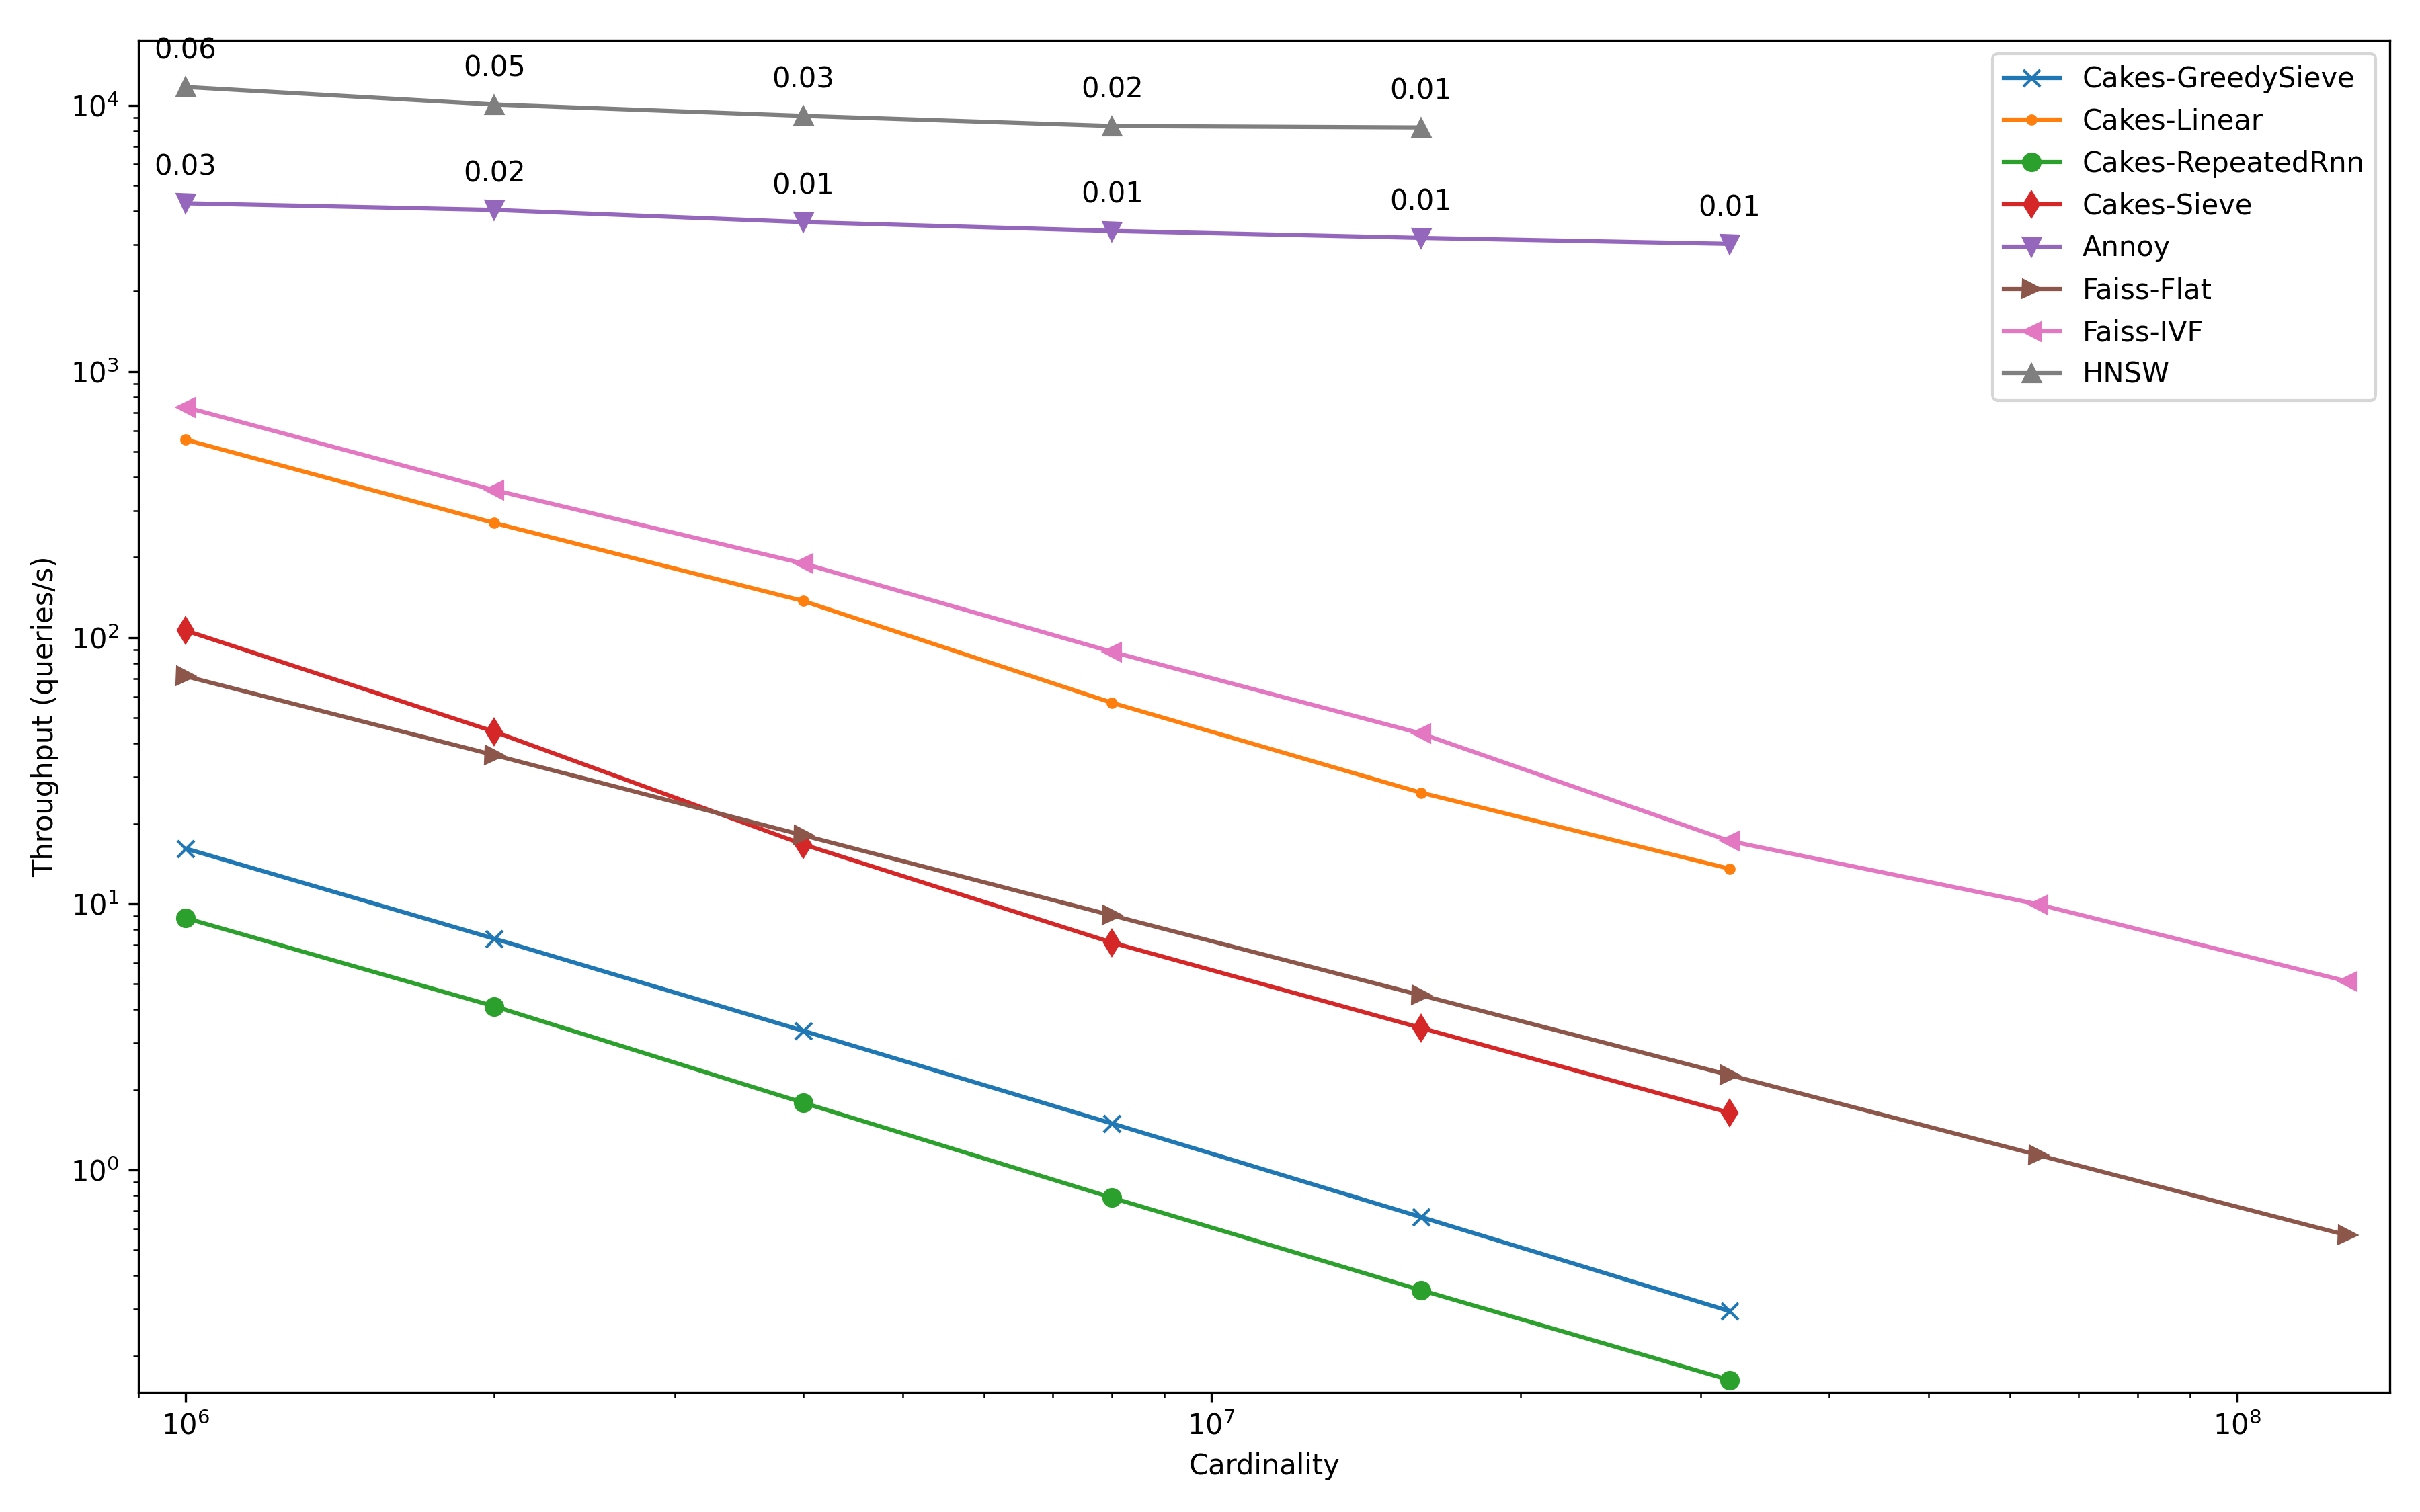
\includegraphics[width=3.4in]{plots/random-1000000-128-knn-10.png}
%     \caption{
%         Algorithm performance by cardinality multiplier on a random dataset for $k=10$.
%     }
%     \label{fig:results:random-scaling}
% \end{figure}


% We did not run any of the competitor's algorithms.
% We lifted the reported numbers from the ann-benchmarks site and their interactive plots.
% We made sure to use the same AWS instance as they did so it is a fair comparison.

% Tables \ref{table:results:ann-10} and \ref{table:results:ann-100} show the results of our benchmarks against FAISS, bruteforce-blas, and HNSW.
% The throughput values for these algorithms comes from the ANN benchmarks website's interactive plots, from which we can assess the throughput of each algorithm at a given recall value.

% We report the highest throughput value for each algorithm at a recall value of 1.0.
% We report the mean and median speedup factor of CAKES over each algorithm.
% For $k= 10$, we report a mean $7,654 \times$ (median $1,200 \times$) speedup over faiss-ivf, a mean $11,325 \times$ (median $2,821 \times$) speedup over bruteforce-blas, and a mean $485 \times$ (median $417 \times$) speedup over HNSW. 
% For $k=100$, we report a mean $4,479 \times$ (median $3,456 \times$) speedup over faiss-ivf, a mean $16,010 \times$ (median $13,548 \times$) speedup over bruteforce-blas, and a mean $403 \times$ (median $372 \times$) speedup over HNSW.

% For all datasets benchmarked in this manuscript, the auto-tuning method selected repeated $\rho$-nearest neighbor (Section~\ref{subsubsec:methods:knn-search:repeated-rnn}).

% We note that the mean and median speedup factors differ significantly for all methods, which suggests that the speedup factor is heavily dataset-dependent;
% in particular, across all algorithms, and both values of $k$, CAKES exhibits particularly high speedup factors with SIFT and GIST, under Euclidean distance.
% As GIST was designed to be a difficult dataset for classifiers~\cite{Lee2019PracticalLP}, CAKES's strong performance with this dataset is particularly encouraging.
% Further investigation of CAKES's performance on other challenging or adversarial datasets is warranted. 




\begin{table*}[!t]
    % \renewcommand{\arraystretch}{1.15}
    \caption{Runtime performance (queries per second) and recall of CAKES vs. other methods on the fashion-mnist dataset. We use 1.000* to denote that the recall is imperfect, but rounds to 1.000 when we consider only three decimal places.}
    \label{table:results:ann-fashion}
    \vskip 0.15in
    \begin{center}
        \begin{small}
            \begin{sc}
                \begin{tabular}{|l|p{1cm}|p{1cm}|p{1cm}|p{1cm}|p{1cm}|p{1cm}|p{1cm}|p{1cm}|p{1cm}|p{1cm}|}
                    \hline
                    \textbf{Scale}  & \multicolumn{2}{|c|}{\textbf{hnsw}} & \multicolumn{2}{|c|}{\textbf{annoy}} & \multicolumn{2}{|c|}{\textbf{faiss-flat}} & \multicolumn{2}{|c|}{\textbf{faiss-ivf}}  & \multicolumn{2}{|c|}{\textbf{CAKES}} \\
                    \hline
                    &             QPS & Recall        & QPS & Recall      & QPS & Recall       & QPS & Recall     & QPS & Recall    \\
                    \hline
                    1 & 13330.275 & 0.954 & 2191.849 & 0.950 & 212.602 & 1.000 & 2009.483 & 1.000 & 2167.365 & 1.000 \\
                    \hline
                    2 & 13822.528 & 0.803 & 2118.513 & 0.927 & 106.372 & 1.000 & 939.169 & 1.000 & 1141.225 & 1.000 \\
                    \hline
                    4 & 16648.524 & 0.681 & 2043.628 & 0.898 & 53.077 & 1.000 & 461.016 & 0.997 & 982.117 & 1.000 \\
                    \hline
                    8 & 16785.981 & 0.525 & 1925.593 & 0.857 & 26.577 & 1.000 & 225.827 & 0.995 & 1179.813 & 1.000 \\
                    \hline
                    16 & 18717.175 & 0.494 & 1841.863 & 0.862 & 13.292 & 1.000 & 116.960 & 0.991 & 1201.409 & 1.000 \\
                    \hline
                    32 & 15597.778 & 0.542 & 1850.943 & 0.775 & 6.647 & 1.000 & 59.148 & 0.985 & 1157.667 & 1.000 \\
                    \hline
                    64 & 14997.277 & 0.378 & 1787.142 & 0.677 & 3.324 & 1.000 & 26.068 & 0.968 & 1102.849 & 1.000 \\
                    \hline
                    128 & 14866.019 & 0.357 & 1659.660 & 0.538 & 1.662 & 1.000 & 13.265 & 0.964 & 1039.607 & 1.000 \\
                    \hline
                    256 & -- & -- & 1597.264 & 0.592 & 0.831 & 1.000 & 6.650 & 0.962 & 1058.972 & 1.000 \\
                    \hline
                    512 & -- & -- & 1826.362 & 0.581 & 0.416 & 1.000 & 3.563 & 0.949 & 1035.260 & 1.000 \\
                    \hline
                \end{tabular}
            \end{sc}
        \end{small}
    \end{center}
    \vskip -0.1in
\end{table*}


\begin{table*}[!t]
    % \renewcommand{\arraystretch}{1.15}
    \caption{Runtime performance (queries per second) and recall of CAKES vs. other methods on the glove-25 dataset. We use 1.000* to denote that the recall is imperfect, but rounds to 1.000 when we consider only three decimal places.}
    \label{table:results:ann-fashion}
    \vskip 0.15in
    \begin{center}
        \begin{small}
            \begin{sc}
                \begin{tabular}{|l|p{1cm}|p{1cm}|p{1cm}|p{1cm}|p{1cm}|p{1cm}|p{1cm}|p{1cm}|p{1cm}|p{1cm}|}
                    \hline
                    \textbf{Scale}  & \multicolumn{2}{|c|}{\textbf{hnsw}} & \multicolumn{2}{|c|}{\textbf{annoy}} & \multicolumn{2}{|c|}{\textbf{faiss-flat}} & \multicolumn{2}{|c|}{\textbf{faiss-ivf}}  & \multicolumn{2}{|c|}{\textbf{CAKES}} \\
                    \hline
                    &             QPS & Recall        & QPS & Recall      & QPS & Recall       & QPS & Recall     & QPS & Recall    \\
                    \hline
                    1 & 22755.175 & 0.801 & 2829.338 & 0.835 & 278.176 & 1.000 & 2378.006 & 1.000 & 722.326 & 1.000 \\
                    \hline
                    2 & 23792.690 & 0.607 & 2701.804 & 0.832 & 139.414 & 1.000 & 1188.398 & 1.000 & 574.516 & 1.000 \\
                    \hline
                    4 & 24990.630 & 0.443 & 2609.474 & 0.839 & 69.813 & 1.000 & 619.241 & 1.000 & 625.208 & 1.000 \\
                    \hline
                    8 & 27843.055 & 0.294 & 2514.357 & 0.834 & 34.878 & 1.000 & 302.683 & 1.000 & 592.699 & 1.000 \\
                    \hline
                    16 & 31114.062 & 0.213 & 2225.654 & 0.885 & 17.437 & 1.000 & 150.971 & 1.000 & 549.073 & 1.000 \\
                    \hline
                    32 & 32423.543 & 0.178 & 2008.537 & 0.764 & 8.701 & 1.000 & 74.016 & 0.999 & 475.266 & 1.000 \\
                    \hline
                    64 & -- & -- & 1990.317 & 0.631 & 4.362 & 1.000 & 37.735 & 0.997 & 461.066 & 1.000 \\
                    \hline
                    128 & -- & -- & -- & -- & 2.176 & 1.000 & 18.960 & 0.998 & 440.758 & 1.000 \\
                    \hline
                    256 & -- & -- & -- & -- & 1.067 & 1.000 & 9.472 & 0.998 & 422.591 & 1.000 \\
                    \hline
                    % 512 & -- & -- & -- & -- & 0.544 & 1.000 & 4.499 & 0.996 & 0.000 & 0.000 \\
                    % \hline
                \end{tabular}
            \end{sc}
        \end{small}
    \end{center}
    \vskip -0.1in
\end{table*}

\begin{table*}[!t]
    % \renewcommand{\arraystretch}{1.15}
    \caption{Runtime performance (queries per second) and recall of CAKES vs. other methods on the sift dataset. We use 1.000* to denote that the recall is imperfect, but rounds to 1.000 when we consider only three decimal places.}
    \label{table:results:ann-fashion}
    \vskip 0.15in
    \begin{center}
        \begin{small}
            \begin{sc}
                \begin{tabular}{|l|p{1cm}|p{1cm}|p{1cm}|p{1cm}|p{1cm}|p{1cm}|p{1cm}|p{1cm}|p{1cm}|p{1cm}|}
                    \hline
                    \textbf{Scale}  & \multicolumn{2}{|c|}{\textbf{hnsw}}  & \multicolumn{2}{|c|}{\textbf{annoy}} & \multicolumn{2}{|c|}{\textbf{faiss-flat}} & \multicolumn{2}{|c|}{\textbf{faiss-ivf-flat}}  & \multicolumn{2}{|c|}{\textbf{CAKES}} \\
                    \hline
                    &             QPS & Recall        & QPS & Recall      & QPS & Recall       & QPS & Recall    & QPS & Recall    \\
                    \hline
                    1 & 19330.282 & 0.782 & 3977.432 & 0.686 & 72.610 & 1.000 & 697.809 & 1.000 & 551.894 & 1.000 \\
                    \hline
                    2 & 20319.372 & 0.552 & 3800.401 & 0.614 & 36.237 & 1.000 & 329.950 & 1.000 & 265.615 & 1.000 \\
                    \hline
                    4 & 21765.007 & 0.394 & 3686.606 & 0.637 & 18.152 & 1.000 & 165.175 & 1.000 & 142.545 & 1.000 \\
                    \hline
                    8 & 24796.528 & 0.298 & 3582.099 & 0.710 & 9.077 & 1.000 & 77.187 & 1.000 & 79.353 & 1.000 \\
                    \hline
                    16 & 26760.717 & 0.210 & 3498.893 & 0.690 & 4.539 & 1.000 & 39.809 & 1.000 & 81.172 & 1.000 \\
                    \hline
                    32 & 27522.668 & 0.193 & 3435.058 & 0.639 & 2.269 & 1.000 & 20.910 & 0.999 & 78.124 & 1.000 \\
                    \hline
                    64 & -- & -- & 3391.916 & 0.678 & 1.135 & 1.000 & 8.867 & 0.997 & 74.344 & 1.000 \\
                    \hline
                    128 & -- & -- & 3363.965 & 0.643 & 0.566 & 1.000 & 4.786 & 0.993 & 68.005 & 1.000 \\
                    \hline
                \end{tabular}
            \end{sc}
        \end{small}
    \end{center}
    \vskip -0.1in
\end{table*}


\begin{table*}[!t]
    % \renewcommand{\arraystretch}{1.15}
    \caption{Runtime performance (queries per second) and recall of CAKES vs. other methods on a random dataset. We use 1.000* to denote that the recall is imperfect, but rounds to 1.000 when we consider only three decimal places.}
    \label{table:results:ann-fashion}
    \vskip 0.15in
    \begin{center}
        \begin{small}
            \begin{sc}
                \begin{tabular}{|l|p{1cm}|p{1cm}|p{1cm}|p{1cm}|p{1cm}|p{1cm}|p{1cm}|p{1cm}|p{1cm}|p{1cm}|}
                    \hline
                    \textbf{Scale}  & \multicolumn{2}{|c|}{\textbf{hnsw}}  & \multicolumn{2}{|c|}{\textbf{annoy}} & \multicolumn{2}{|c|}{\textbf{faiss-flat}} & \multicolumn{2}{|c|}{\textbf{faiss-ivf-flat}}  & \multicolumn{2}{|c|}{\textbf{CAKES}} \\
                    \hline
                    &             QPS & Recall        & QPS & Recall      & QPS & Recall       & QPS & Recall    & QPS & Recall    \\
                    \hline
                    1 & 11713.738 & 0.060 & 4283.182 & 0.028 & 71.575 & 1.000 & 733.821 & 1.000 & 553.948 & 1.000 \\
                    \hline
                    2 & 10061.864 & 0.048 & 4043.999 & 0.021 & 36.157 & 1.000 & 358.083 & 1.000 & 269.314 & 1.000 \\
                    \hline
                    4 & 9120.868 & 0.031 & 3639.337 & 0.014 & 18.072 & 1.000 & 189.802 & 1.000 & 137.236 & 1.000 \\
                    \hline
                    8 & 8352.077 & 0.022 & 3371.923 & 0.013 & 9.036 & 1.000 & 88.375 & 1.000 & 56.871 & 1.000 \\
                    \hline
                    16 & 8250.619 & 0.008 & 3174.156 & 0.006 & 4.531 & 1.000 & 43.613 & 1.000 & 26.136 & 1.000 \\
                    \hline
                    32 & -- & -- & 3013.970 & 0.007 & 2.270 & 1.000 & 17.201 & 1.000 & 13.534 & 1.000 \\
                    % \hline
                    % 64 & -- & -- & -- & -- & 1.135 & 1.000 & 9.939 & 1.000 & 0.000 & 0.000 \\
                    % \hline
                    % 128 & --& -- & -- & -- & 0.567 & 1.000 & 5.106 & 1.000 & 0.000 & 0.000 \\
                    \hline
                \end{tabular}
            \end{sc}
        \end{small}
    \end{center}
    \vskip -0.1in
\end{table*}

% \begin{table*}[!t]
%     % \renewcommand{\arraystretch}{1.15}
%     \caption{Runtime performance (queries per second) of CAKES and Speedup Factor over Naive Linear Search, $k=10$}
%     \label{table:results:ann-alt-10}
%     \vskip 0.15in
%     \begin{center}
%         \begin{small}
%             \begin{sc}
%                 \begin{tabular}{|l|l|l|l|l|}
%                     \hline
%                     \textbf{Dataset} & \textbf{CAKES Throughput} & \textbf{Speedup Factor over Linear} \\
%                     \hline
%                     deep-image       & 232.1                     & 37.2      \\
%                     \hline
%                     mnist            & 129,300                   & 101.9      \\
%                     \hline
%                     glove-50         & 10,950                    & 12.28      \\
%                     \hline 
%                     glove-200        & 2,290                     & 8.55     \\
%                     \hline
%                     lastfm           & 13,950                    & 4.55           \\
%                     \hline
%                 \end{tabular}
%             \end{sc}
%         \end{small}
%     \end{center}
%     \vskip -0.1in
% \end{table*}


% \begin{table*}[!t]
%     % \renewcommand{\arraystretch}{1.15}
%     \caption{Runtime performance (queries per second) of CAKES and Speedup Factor over Naive Linear Search, $k=100$}
%     \label{table:results:ann-alt-100}
%     \vskip 0.15in
%     \begin{center}
%         \begin{small}
%             \begin{sc}
%                 \begin{tabular}{|l|l|l|l|l|l|}
%                     \hline
%                     \textbf{Dataset} & \textbf{CAKES Throughput} & \textbf{Speedup Factor over Linear} \\
%                     \hline
%                     deep-image        & 157.3                    & 25.74                               \\                            
%                     \hline
%                     mnist             & 71,090                   & 56.63                               \\
%                     \hline
%                     glove-50          & 8,867                    & 9.84                                \\
%                     \hline 
%                     glove-200         & 2,264                    & 8.49                                \\
%                     \hline
%                     lastfm            & 13,950                   & 4.55                                \\
%                     \hline
%                 \end{tabular}
%             \end{sc}
%         \end{small}
%     \end{center}
%     \vskip -0.1in
% \end{table*}
